\documentclass[a4paper,10pt]{article}
\usepackage[utf8]{inputenc}
\usepackage{graphicx}
\usepackage{xcolor}
\usepackage{amsmath}   
\usepackage{amssymb}
\usepackage{listings}
\usepackage{framed} 
\usepackage{scrtime}
\usepackage[ngerman]{babel} %deutsches Datum
\usepackage[bookmarksopen=true,colorlinks,linkcolor = black]{hyperref}

\usepackage{xcolor}
\definecolor{codecolor}{RGB}{245,222,179}
\definecolor{codegreen}{rgb}{0,0.6,0}
\definecolor{codegray}{rgb}{0.5,0.5,0.5}
\definecolor{codepurple}{rgb}{0.58,0,0.82}
\definecolor{backcolour}{rgb}{0.95,0.95,0.92}
%Stelle Quellcode ein
\lstset{
    backgroundcolor=\color{backcolour},   
    commentstyle=\color{codegreen},
    keywordstyle=\color{magenta},
    numberstyle=\tiny\color{codegray},
    stringstyle=\color{codepurple},
    basicstyle=\footnotesize,    
    language=C++,
    numbers=left,
    captionpos=b,
    frame=shadowbox,
    showspaces=false,
    showstringspaces=false,
    showtabs=false,
    breaklines=true,
    escapeinside={(*•}{•*)},
    numbers=left,
    numbersep=5pt,    
    rulesepcolor=\color{gray},
    framexleftmargin=5mm
}

%Dokument breiter machen
\setlength{\oddsidemargin}{-1cm}
\setlength{\evensidemargin}{-1cm}
\setlength{\textwidth}{16cm}

%Codeumgebung farbig machen
\renewcommand\FrameCommand{\fcolorbox{black}{codecolor}} 


\title{\textbf{XML Technologien\\ Projekt: TierstimmenQuiz}}
\date{\today}
\begin{document}

\maketitle
%#################
%     Begin
%#################
\section{Gruppenmitglieder}
    \begin{itemize}
        \item Jakob Warkotsch
        \item Patrick Schumacher
        \item Peter Schiessl
        \item Kordian Gontarska
        \item Alexander Hinze-Hüttl
        \item Lars Parmakerli
    \end{itemize}

\section{Spielprinzip}
    Das TierstimmenQuiz wird vom Benutzer im Browser gespielt.
    Ihm werden nacheinander 10 Fragen gestellt, die er zu beantworten hat.
    Zu Beginn jeder Frage wird eine Tierstimme abgespielt. Der Benutzer muss 
    diese Tierstimme einem von vier vorgeschlagenen Tieren zuordnen.\\
    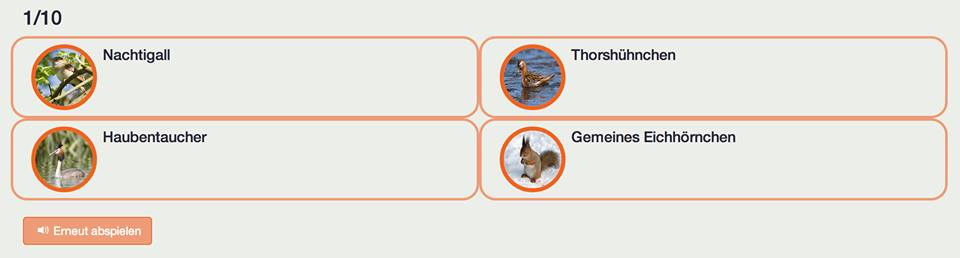
\includegraphics[scale=0.5]{p1}
    Wenn sich der Benutzer für eine Antwort entschieden hat, wird die Frage aufgelöst.
    Es wird der Text und ein Bild angezeigt.\\
    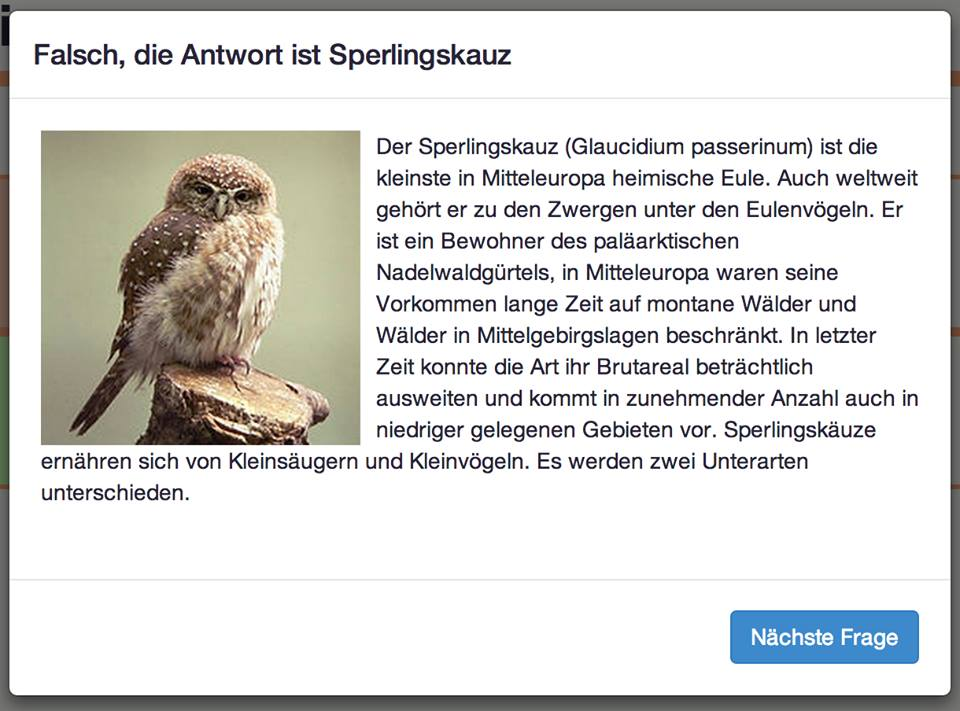
\includegraphics[scale=0.3]{p2}
\section{Projektaufbau}
        \subsection{Download der Daten}
        Zunächst werden Tierstimmen und Informationen von \href{http://offene-naturfuehrer.de/web/Open_Source_Tierstimmen}{Sounddateien der Tierstimmen} runtergeladen und im \texttt{CSV} Format abgelegt.
        
        \subsection{Anreicherung}
            Da \texttt{SPARQL}-Abfragen an einen Trippel Datastore je nach Komplexität des Querys 
            lange dauern können, und wir unabhängig von Serverausfällen dritter 
            sein wollen, werden die Daten zu Beginn mit Informationen
            aus der deutschen DBPedia angereichert. Ein Python Skript ließt 
            die gegrabbten Daten ein und erstellt eine SPARQL Abfrage, um Daten mit Bildern
            der Tiere und den Wiki Texten anzureichern.
            
       \subsection{Aufbereitung}
           Zunächst wird eine XSL Transformation angewendet, um die \texttt{CSV} Daten in
           ein definiertes XML Schema zu überführen.\\
           Anschließend werden defekte Datensätze entfernen. Da es zu einigen Tiernamen aus
           dem Tierstimmenarchiv keinen Wikipediaartikel gibt, existieren zu diesen
           Tieren keine Bilder und keine Wiki Texte.
           
       \subsection{Backend}
           Das Backend basiert auf einem Java Servlet, welches eine Restschnittstelle 
           besitzt. Das Backend hält einen BaseX-Datenbank, welche
           die angereicherten Informationen über die Tiere/Tierstimmen
           beinhaltet. Ein Algorithmus stellt zufällige (Frage-)Datensätze zusammen
           und stellt diese über die Restschnittstelle zur Verfügung.
           
       \subsection{Frontend}
           Das Frontend läuft auf einem Sinatra Webserver und wurde durch HMTL, Javascript und CSS mittels \texttt{Backbone.js} und \texttt{Bootstrap} gestaltet. Es bezieht mittels AJAX-Request die (Frage)Datensätze über die Restschnittstelle des Backends.
           Zudem wird eine mit RDFa-Infomationen angereicherte, statisches HTML Dokument
           zur Verfügung gestellt.
\end{document}